\documentclass[12pt,a4paper]{article}
 
                               
\usepackage[T1]{fontenc} % So we can use pretty T1 fonts
\usepackage{libertine}
 
\usepackage[margin=0.5in]{geometry}
\usepackage{amsmath,amssymb,amsfonts}
\usepackage{graphicx}
\usepackage{textcomp}
\usepackage{soul}
\usepackage{hyperref}
\usepackage{xcolor}
\usepackage{caption}
\usepackage{booktabs}
\usepackage{cancel}
\usepackage{algorithm}
\usepackage{algorithmic}
%\usepackage{helvet}
%\usepackage{courier}
\usepackage{mathtools}
\usepackage{pifont}
\usepackage{dashbox}
\usepackage{xspace}
\usepackage{color}
\usepackage{multirow}
\usepackage{url}
%\usepackage{extsizes}
% the following package is optional:
\usepackage{latexsym}
%\usepackage{mathptmx}
\usepackage{stmaryrd}
\usepackage{enumitem}
\newtheorem{definition}{Definition}
\setlength\parindent{0pt}

\makeatletter
\newcommand\makebig[2]{%
  \@xp\newcommand\@xp*\csname#1\endcsname{\bBigg@{#2}}%
  \@xp\newcommand\@xp*\csname#1l\endcsname{\@xp\mathopen\csname#1\endcsname}%
  \@xp\newcommand\@xp*\csname#1r\endcsname{\@xp\mathclose\csname#1\endcsname}%
}
\makeatother

\makebig{biggg} {3.0}
\makebig{Biggg} {3.5}
\makebig{bigggg}{5.0}
\makebig{Bigggg}{14.0}

\newcommand{\alc}{$\mathcal{ALC}$\xspace}
\newcommand{\el}{$\mathcal{EL}$\xspace}
\newcommand{\sig}{\textsf{sig}\xspace}
%para nao ficar o retangulo em volta dos links, apenas muda a cor dos caracteres
%para nao ficar o retangulo em volta dos links, apenas muda a cor dos caracteres
\hypersetup{ colorlinks,
linkcolor=blue,
filecolor=blue,
urlcolor=blue,
citecolor=blue }

% altera a fonte nas legendas das figuras
%\usepackage[font=small,format=plain,labelfont=bf,up,textfont=times]{caption}
 

\newenvironment{problem}[2][{\color{red}Question}]{\begin{trivlist}
\item[\hskip \labelsep {\bfseries #1}\hskip \labelsep {\bfseries #2.}]}{\end{trivlist}}

\newenvironment{problems}[2][{\color{purple}Question}]{\begin{trivlist}
\item[\hskip \labelsep {\bfseries #1}\hskip \labelsep {\bfseries #2.}]}{\end{trivlist}}

\newenvironment{solution}[2][{\color{blue}Model Solution}]{\begin{trivlist}
\item[\hskip\labelsep {\bfseries #1}\hskip \labelsep {\bfseries #2.}]}{\end{trivlist}}

\setlength{\parskip}{0,3em}  %altera o espaco entre dois paragrafos
\renewcommand{\baselinestretch}{1.1} %altera o espacamento entre as linhas
 
\begin{document}


\title{{\color{blue}KRP --- Assignment 5}}
\author{Instructor: Yizheng Zhao}

 
\maketitle

\textbf{$\star$~\textcolor{gray}{This assignment, due on \underline{\textcolor{blue}{30th June at 23:59}}, contributes to 10\% of the final marks for this course. Please be advised that only Questions 1 --- 5 are mandatory. Nevertheless, students can earn up to one bonus mark by completing Question~6. This bonus mark can potentially augment a student's overall marks but is subject to a maximum total of 100 for the course. By providing bonus marks, we aim to incentivize students to excel in their studies and reward those with a remarkable grasp of the course materials.}}


\begin{problem}{{\color{red}1}}
\textbf{Ontology-Mediated Query Answering (2 marks)}\\
\begin{figure}[ht]
    \centering
    
\includegraphics[width=0.6\columnwidth]{PGBBW.jpeg}
     \label{pic1}
\end{figure}
(1) Consider the database instance $\mathcal{D}_{\textsf{PGBBW}}$ (\textsf{PGBBW} stands for \textsf{Pleasant Goat and Big Big Wolf}) below:

\begin{itemize}
    \item[] \textsf{Sheep(weslie)}\quad\textsf{Sheep(slowy)}\quad\textsf{LazySheep(paddi)}
    \item[] \textsf{Sheep(tibbie)}\quad\textsf{BrownSheep(fitty)}\quad\textsf{Sheep(jonie)}
    \item[] \textsf{Wolf(wolffy)}\quad\textsf{Wolf(wolnie)}\quad\textsf{Wolf(wilie)}
    \item[] \textsf{hasFriend(weslie, slowy)}\quad\textsf{hasFriend(tibbie, jonie)}
    \item[] \textsf{hasEnemy(paddi, wolffy)}\quad\textsf{hasWife(wolffy, wolnie)}\quad\textsf{hasSon(wolnie, wilie)}
\end{itemize}


\noindent We query $\mathcal{D}_{\textsf{PGBBW}}$ under closed world assumption (relational database) and under open world assumption. Recall that under the closed world assumption we consider the interpretation $\mathcal{I}:=\mathcal{I}_{\mathcal{D}_{\textsf{PGBBW}}}$ defined as follows:

\begin{itemize}
    \item[] $\Delta^{\mathcal{I}}=\{\textsf{weslie, slowy, paddi, tibbie, fitty, jonie, wolffy, wolnie, wilie}\}$
    \item[] $\textsf{Sheep}^{\mathcal{I}}=\{\textsf{weslie, slowy, tibbie, jonie}\}$
    \item[] $\textsf{LazySheep}^{\mathcal{I}}=\{\textsf{paddi}\}$
    \item[] $\textsf{BrownSheep}^{\mathcal{I}}=\{\textsf{fitty}\}$
    \item[] $\textsf{Wolf}^{\mathcal{I}}=\{\textsf{wolffy, wolnie, wilie}\}$
    \item[] $\textsf{hasFriend}^{\mathcal{I}}=\{(\textsf{weslie, slowy}),(\textsf{tibbie, jonie})\}$
    \item[] $\textsf{hasEnemy}^{\mathcal{I}}=\{(\textsf{paddi, wolffy})\}$
    \item[] $\textsf{hasWife}^{\mathcal{I}}=\{(\textsf{wolffy, wolnie})\}$
    \item[] $\textsf{hasSon}^{\mathcal{I}}=\{(\textsf{wolnie, wilie})\}$
\end{itemize}


Consider the following non-Boolean queries $F_{i}$:

\begin{enumerate}
    \item $F_{1}(x)=\textsf{Wolf}(x)$ 
    \item $F_{2}(x)=\neg\textsf{Sheep}(x)$ 
    \item $F_{3}(x,y)=\textsf{hasFriend}(x,y)$ 
    \item $F_{4}(x)=\textsf{Sheep}(x)\wedge\neg\textsf{hasFriend}(x,\textsf{jonie})$
\end{enumerate}

For each $F_{i}$, give

\begin{itemize}
    \item[-] for closed world assumption: \textsf{answer($F_{i}$,$\mathcal{D}_{\textsf{PGBBW}}$)};
    \item[-] for open world assumption: \textsf{certanswer($F_{i}$,$\mathcal{D}_{\textsf{PGBBW}}$)}. 
\end{itemize}


(2). Following (1), consider now the TBox $\mathcal{T}$ given as:
\begin{align*}
    \textsf{LazySheep} & \sqsubseteq \textsf{Sheep}\\
    \textsf{LazySheep}\sqcap\textsf{BrownSheep} & \sqsubseteq\bot\\
    \textsf{Sheep}\sqcap\textsf{Wolf} & \sqsubseteq\bot\\
    \top & \sqsubseteq\forall\textsf{hasFriend.Sheep}\\
    \exists\textsf{hasFriend.Sheep} & \sqsubseteq\textsf{Sheep}\\
    \textsf{Sheep} & \sqsubseteq\exists\textsf{hasFriend.}\top
\end{align*}
Fill in the table below with the answers ``Yes'', ``No'' or ``Don't know'' to the Boolean queries.

\begin{table}[ht] 
\begin{center}
\label{BooleanQueries}
\scalebox{0.71}{
\begin{tabular}{|c|c|c|c|}  

\hline 
~Query~& ~Answer for $\mathcal{I}$~&~Certain Answer for $\mathcal{D}_{\textsf{PGBBW}}$~&~Certain Answer for $(\mathcal{T}, \mathcal{D}_{\textsf{PGBBW}})$~\\
\hline\hline
\textsf{LazySheep(paddi)}&    &  & \\
\hline
\textsf{LazySheep(fitty)}&    &  & \\
\hline
\textsf{Sheep(paddi)}&    &   & \\
\hline
$\neg$\textsf{Sheep(paddi)}&    &  & \\
\hline
\textsf{BrownSheep(wilie)}&   &   & \\
\hline
\textsf{Wolf(fitty)}&   &   & \\
\hline
\textsf{$\exists$hasFriend.$\top$(fitty)} &   &  & \\
\hline
\textsf{$\forall$hasFriend.$\top$(wolffy)}&    &  &  \\
\hline
\textsf{$\forall$hasFriend.$\exists$hasFriend.$\top$(wolnie)}&    &   & \\
\hline
\textsf{$\exists$hasFriend.$\forall$hasFriend.$\top$(jonie)}&    &  & \\
\hline
\end{tabular}
}
\end{center}
\end{table}


\end{problem}



\begin{problem}{{\color{red}2}}
\textbf{Computing $\mathcal{I}_{\mathcal{T},\mathcal{A}}$ in $\mathcal{EL}$}\\
Consider the following $\mathcal{EL}$ TBox $\mathcal{T}$:
\begin{align*}
    \textsf{Vocalist} & \sqsubseteq \exists\textsf{plays\_for.Band}\\
    \textsf{Guitarist} & \sqsubseteq \exists\textsf{plays\_for.Band}\\
    \textsf{Bassist} & \sqsubseteq \exists\textsf{plays\_for.Band}\\
    \textsf{Drummer} & \sqsubseteq \exists\textsf{plays\_for.Band}\\
    \textsf{LeadGuitarist} & \sqsubseteq\textsf{Guitarist}\\
    \textsf{RhythmGuitarist} & \sqsubseteq\textsf{Guitarist}\\
    \textsf{Band} & \sqsubseteq\exists\textsf{captained\_by.Captain}\\
    \textsf{Band} & \sqsubseteq\exists\textsf{managed\_by.Manager}\\
    \textsf{Manager} & \sqsubseteq \exists\textsf{managed\_by.Manager}
\end{align*}
\begin{figure}[ht]
    \centering
    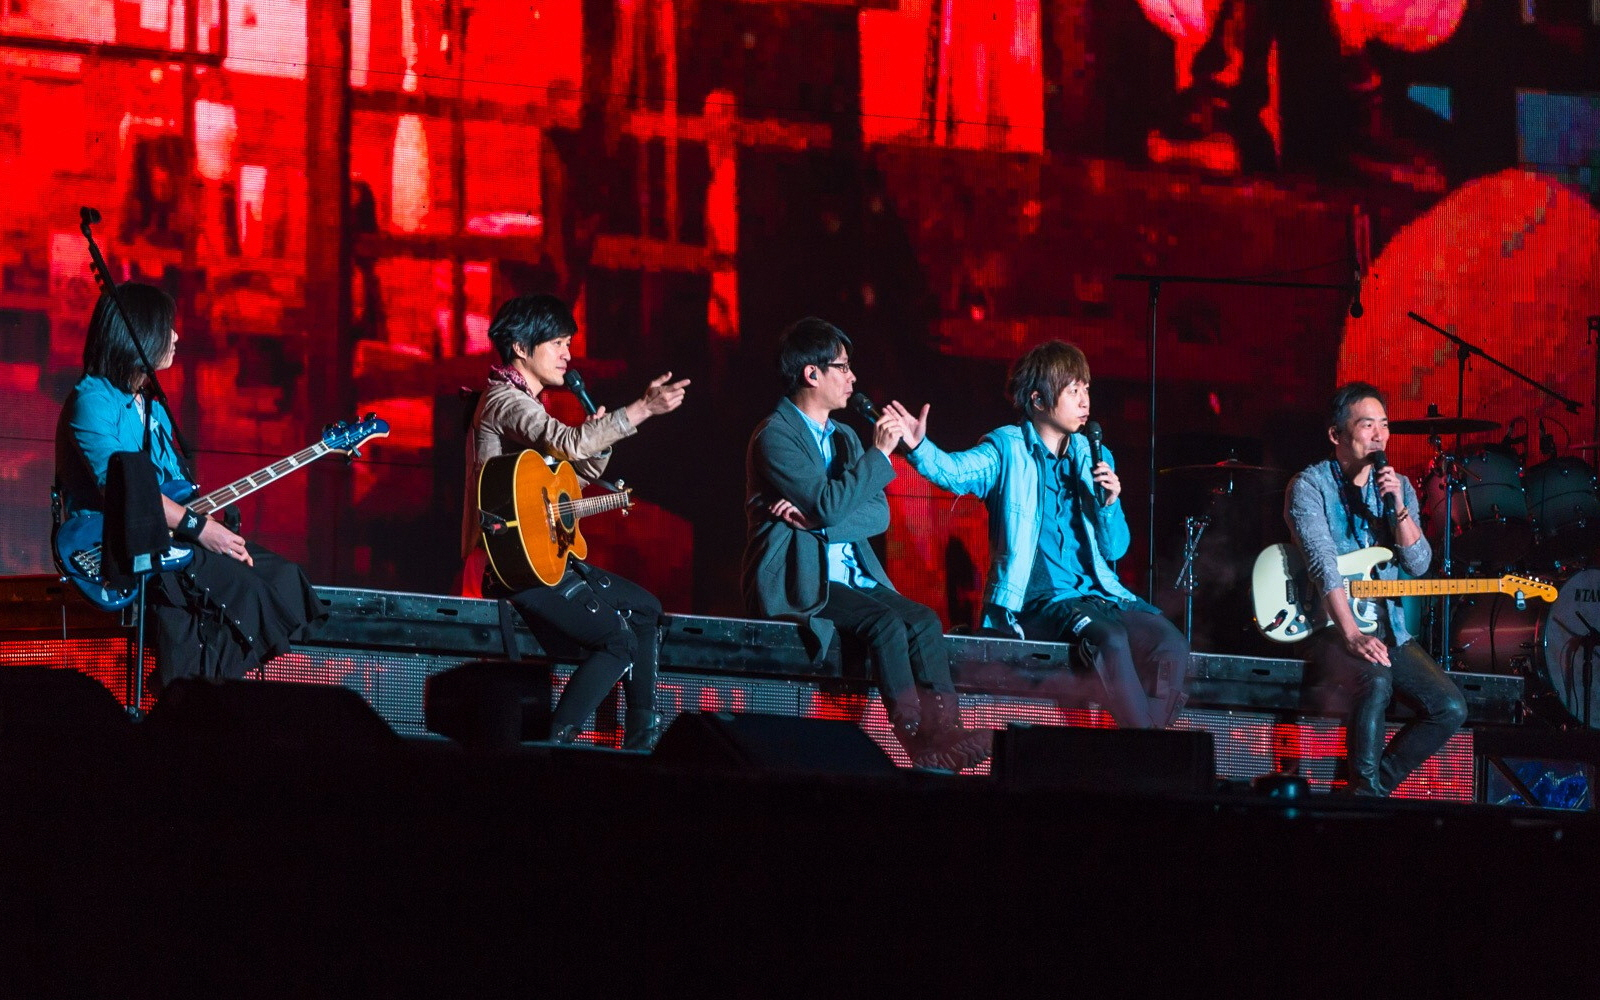
\includegraphics[width=0.6\columnwidth]{mayday.jpg}
     \label{pic2}
\end{figure}
and the following ABox $\mathcal{A}$:
\begin{align*}
    \textsf{Captain(Monster)}\quad &\textsf{Vocalist(Ashin)}\\
    \textsf{LeadGuitarist(Monster)}\quad & \textsf{Bassist(Masa)}\\
    \textsf{RhythmGuitarist(Stone)}\quad & \textsf{Drummer(Ming)}\\
    \textsf{Band(Mayday)}\quad & \textsf{managed\_by(Mayday, Amuse)}
\end{align*}~\\~\\~\\~\\
\begin{itemize}
\item[-] Compute the interpretation $\mathcal{I}_{\mathcal{T},\mathcal{A}}$ as described in the slides.
\item[-] For $\mathcal{EL}$ concept queries, we know that $\mathcal{I}_{\mathcal{T},\mathcal{A}}$ gives the answer ``Yes'' iff $(\mathcal{T}, \mathcal{A})$ gives the certain answer ``Yes''. Check this for the following queries:
\begin{enumerate}
\item \textsf{$\exists$plays\_for.Band(Ashin);}
\item \textsf{$\exists$managed\_by.Manager(Masa);}
\item \textsf{$\exists$plays\_for.$\exists$captained\_by.Captain(Monster);}
\item \textsf{$\exists$plays\_for.$\exists$managed\_by.Manager(Ming).}
\end{enumerate}
\item[-] For more complex queries, $\mathcal{I}_{\mathcal{T},\mathcal{A}}$ can give the answer ``Yes'' even if $(\mathcal{T}, \mathcal{A})$ does not give the certain answer ``Yes''. Check this for:
\begin{enumerate}
\item $F(x,y)=\exists z.(\textsf{plays\_for}(x,z)\wedge\textsf{plays\_for}(y,z))$.
\item $F=\exists x.\textsf{managed\_by}(x,x)$.
\end{enumerate}
\end{itemize}
\end{problem}


\begin{problem}{{\color{red}3}}
\textbf{SQL and Conjunctive Queries (2 marks)}\\
Consider the following database $\mathcal{D}$ consisting of the following tables:
\begin{table}[ht] 
\begin{center}
\label{table1}
\scalebox{1.0}{
\begin{tabular}{|c|c|}  
Person: & \\
\hline 
ID~& Name \\
\hline
\textsf{2101}&  \textsf{Jay\_Chou}\\

\textsf{2102}&  \textsf{Jolin\_Tsai}\\

\textsf{2103}&  \textsf{Stefanie\_Sun}\\

\textsf{2104}&  \textsf{Ta-yu\_Lo}\\
\hline
\end{tabular}
}\scalebox{1.0}{
\begin{tabular}{|c|c|}  
Enrollment: & \\
\hline 
StudentID~& Since \\
\hline
\textsf{2102}&  \textsf{2020}\\

\textsf{2103}&  \textsf{2021}\\

\textsf{2104}&  \textsf{2020}\\

& \\
\hline
\end{tabular}
}\scalebox{1.0}{\begin{tabular}{|c|c|} 
Attendance: &\\
\hline 
StudentID~& CourseID \\
\hline
\textsf{2101}&  \textsf{30000160}\\

\textsf{2102}&  \textsf{30000160}\\

\textsf{2102}&  \textsf{30000170}\\

\textsf{2103}&  \textsf{30000150}\\
\hline
\end{tabular}
}\scalebox{1.0}{\begin{tabular}{|c|c|}  
Course: &\\
\hline 
ID~& Title \\
\hline
\textsf{30000150}&  \textsf{ML}\\

\textsf{30000160}&  \textsf{KRP}\\

\textsf{30000170}&  \textsf{NLP}\\

&  \\
\hline
\end{tabular}
}
\end{center}
\end{table}
\begin{itemize}
    \item[-] Define the finite first-order interpretation $\mathcal{I}_{\mathcal{D}}$ corresponding to $\mathcal{D}$. 
    \item[-] Reformulate each of the following SQL queries $Q$ into first-order queries $f_{Q}$, and identify which of them are conjunctive queries.
    \item[-] Answer $Q$ in the context of $\mathcal{D}$ and $f_{\mathcal{Q}}$ in the context of $\mathcal{I}_{\mathcal{D}}$.
    \item[]\begin{itemize}
    \item[1.] \textsf{SELECT} $\ast$ \textsf{FROM} Person
    \item[2.] \textsf{SELECT} Person.Name \textsf{FROM} Person, Attendance, Course\\
       \text{\textsf{WHERE} Person.ID} = \text{Attendance.PersonID}\\
       \text{~~~~~\textsf{AND} Course.ID} = \text{Attendance.CourseID}\\
       \text{~~~~~\textsf{AND} Course.Title} = ``\textsf{KRP}''
    \item[3.] \textsf{SELECT} Person.Name \textsf{FROM} Person, Enrollment\\
       \text{\textsf{WHERE} Person.ID} = \text{Enrollment.PersonID}\\
       \textsf{AND NOT EXISTS (}\\
       \text{~~~~~\textsf{SELECT}} $\ast$ \textsf{FROM} Attendance\\
       \text{~~~~~\textsf{WHERE}} Person.ID = Attendance.PersonID\textsf{)}
\end{itemize}
\end{itemize}

\end{problem}


\begin{problem}{{\color{red}4}}
\textbf{Certain Answers in $\mathcal{ALC}$ Contexts (2 marks)}\\
Consider the following $\mathcal{ALC}$ knowledge base $\mathcal{K}:=(\mathcal{T},\mathcal{A})$ with:
\begin{align*}
    \mathcal{T} := & \{\textsf{$\textsf{X}\sqsubseteq Y, Y\sqsubseteq\exists r.X, X\sqsubseteq\forall r.Y, \forall r.X\sqsubseteq Y, W\equiv\neg V, \exists r.Y\sqsubseteq\neg V$}\}\\
    \mathcal{A} := & \{\text{(Jay\_Chou, Jolin\_Tsai)} : r, \text{(Jolin\_Tsai, Stefanie\_Sun)} : r, \text{(Stefanie\_Sun, Jay\_Chou)} : r,\\
    & \text{\textcolor{white}{\{}(Jolin\_Tsai, Jolin\_Tsai)} : r, \text{(Stefanie\_Sun, Stefanie\_Sun)} : r, \text{Stefanie\_Sun} : X\}
\end{align*}
\begin{itemize}
    \item[-] Compute the certain answers to the following conjunctive queries in the context of $\mathcal{A}$.
    \item[-] Compute the certain answers to the following conjunctive queries in the context of $\mathcal{K}$.
    \item[]\begin{itemize}
        \item[1.] $r(x, y)\wedge Y(y)$
        \item[2.] $\exists y(r(x, y)\wedge Y(y))$
        \item[3.] $\exists x,y(r(x, y)\wedge r(y, x))$
        \item[4.] $\exists z,w(r(x, y)\wedge r(y, z)\wedge r(z, x)\wedge r(z, w)\wedge W(w))$
    \end{itemize}
\end{itemize}

\end{problem}

\begin{problem}{{\color{red}5}}
\textbf{CW5: Implementing Ontology Queries (2 marks)}\\
CW5 focuses on implementing an OWL-based querying system. Your primary task involves querying the reasoner for sub-classes, equivalent classes, and instances, then storing these results in a QueryResult object. Within the Java class CW5, you are expected to implement specific methods. Please ensure you do not modify any classes other than CW5, as this is the only class you may submit. To evaluate your implementation, you can utilize the provided classes, App.java and PizzaOrderingSystemApp.java. These classes provide a user-friendly way to verify your code's correctness. You can run these classes in Eclipse (or your preferred IDE) by clicking the small white and green arrow icon when the class is open. For a more direct approach, consider using the pre-implemented unit tests to gauge your progress. Note that passing these unit tests does not guarantee a perfect score, as additional tests will be used to assess your solution more comprehensively. Upon completing the assignment, please compress your CW5.java into a zip file for submission. Good luck!
\begin{enumerate}
\item {\textsf{public Set$<$QueryResult$>$ performQuery (OWLClassExpression exp, Query Type type) \{...\}}}\\
This method takes in an arbitrary expression in OWL, like ``Person and hasBirthYear value 1964'' or ``hasTopping some MeatTopping'' and queries the ontology for the following three types of knowledge:\\
EquivalentClasses: you are asked to return all those (named) classes that are equivalent to the expression (exp), using the (already fully initialized) reasoner.\\
Sub-classes: return all those classes that are (named) sub-classes of the expression, using the reasoner.\\
Instances: return all those individuals that are instances of the expression, using the reasoner.\\
Query results are stored in query result objects. These are created for example as follows:\\
{\textsf{QueryResult qr = new QueryResult(ind, false, type);}}\\
Note that you need to include the information whether the inference is direct or indirect. Example: Given three classes with A subclass B subclass C, then A is a direct subclass of B and B is a direct subclass of C, but A is an indirect subclass of C (through B!). In order to solve this problem, you will query the reasoner for direct and indirect sub-class separately. After creating the QueryResult, add it to the provided set.
\item {\textsf{public Boolean isValidPizza (OWLClassExpression exp) \{...\};}}\\
In this method, you check whether the supplied class expression exp is a valid pizza expression, i.e., whether it is inferred to be a Pizza.
\item {\textsf{public Set$<$QueryResult$>$ filterNamedPizzas (Set$<$QueryResult$>$ results) \{...\};}}\\
This question is similar to the one before, only that you are asked to filter from a set of results those that correspond to NamedPizza's, such as Margherita or AmericanHot.
\item {\textsf{public Set$<$OWLClassExpression$>$ getAllSuperClassExpressions (OWLClass ce) \{...\};}}\\
\end{enumerate}
This question requires a bit of thinking. You are asked to query the ontology to gather all available information about the class \textsf{ce}. In order to get an idea of what ``AL'' means, you can open Prot\'eg\'e and look at the ``Classe'' tab. Clicking on a class will reveal its super-classes, equivalent-classes, as well as inherited super-classes (Anonymous Ancestors) and indirect super-classes. Unfortunately, the reasoner will not easily give you access to those. In order to get full marks for this task, it is sufficient to query for all super-classes (direct and indirect, using the reasoner), and somehow find a way to obtain the anonymous super-classes using the ontology directly (that will need a bit of thought, do not despair too quickly). A perfect solution will test, for all sub-expressions in the ontology, whether \textsf{ce} is a sub-concept of it. Attempt this only if you are really confident with the OWL API by now.

\end{problem}


\begin{problems}{{\color{purple}6 (with 1 bonus mark)}}
\textbf{Conservative Extension-based Module Extraction}\\
The design, development, maintenance, reuse, and integration of ontologies are complex tasks. Like software engineers, ontology engineers need to be supported by tools and methodologies that help them to minimize the introduction of errors, i.e., to ensure that ontologies are consistent and do not have unexpected logical consequences. In order to develop this support, important notions from the field of software engineering, such as \emph{module}, \emph{black-box behavior}, and \emph{controlled interaction}, need to be adapted.

For example, consider a scenario where an ontology engineer is building an ontology about research projects, which specifies different types of projects according to the research topic they focus on. While the ontology engineer is an expert on research projects---(s)he knows, for example, that an EUProject is a Project (axiom P3)---(s)he may not be well-versed in the specific topics covered by the projects, particularly when it comes to terms such as ``\textsf{Cystic\_Fibrosis}'' and ``\textsf{Genetic\_Disorder}'' mentioned in axioms P1 and P2. To address this knowledge gap, the engineer decides to leverage the knowledge available in a well-established and widely-used medical ontology $\mathcal{Q}$ containing the axioms \textsf{M1---M5} in Figure~$1$, where the concepts \textsf{Cystic\_Fibrosisis} and \textsf{Genetic\_Disorder} are described.

\begin{figure}[ht]
    \centering
    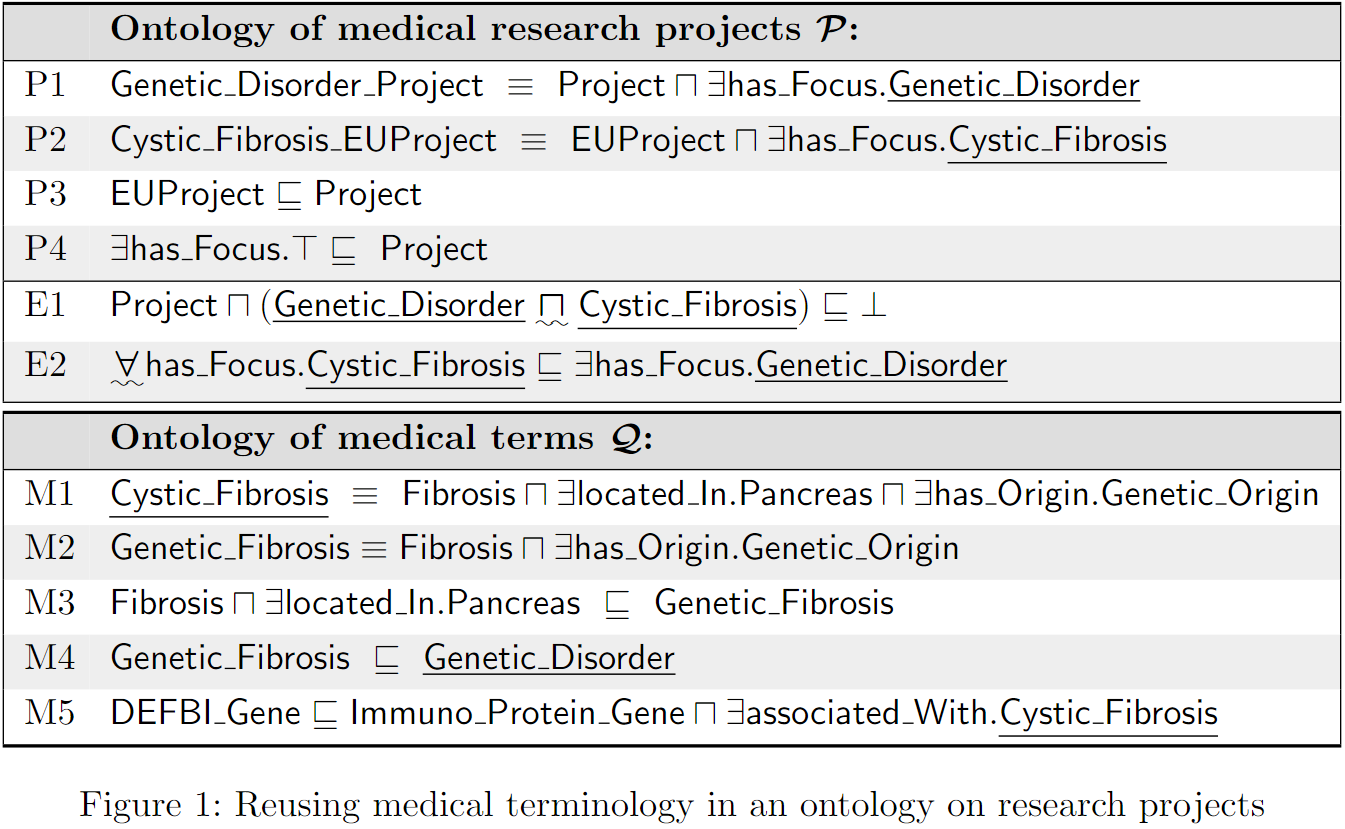
\includegraphics[width=0.75\columnwidth]{ontology.png}
    \label{pic3}
\end{figure}

The most straightforward way to reuse these concepts is to import into $\mathcal{P}$ the ontology $\mathcal{Q}$---that is, to add the axioms from $\mathcal{Q}$ into $\mathcal{P}$ and work with the extended ontology $\mathcal{P}\cup\mathcal{Q}$. Importing additional axioms into an ontology may result in new logical consequences. For example, it is easy to see that axioms \textsf{M1---M4} in $\mathcal{Q}$ imply that every instance of \textsf{Cystic\_Fibrosis} is an instance of \textsf{Genetic\_Disorder}:
\begin{align}
\mathcal{Q}\models\alpha:=\textsf{Cystic\_Fibrosis}\sqsubseteq\textsf{Genetic\_Disorder}
\end{align}
Indeed, the axiom
\begin{align}
\alpha_{1}:=\textsf{Cystic\_Fibrosis}\sqsubseteq\textsf{Genetic\_Fibrosis}
\end{align}follows from the axioms \textsf{M1} and \textsf{M2} as well as from the axioms \textsf{M1} and \textsf{M3}; $\alpha$ follows from the axioms $\alpha_{1}$ and \textsf{M4}. Using $\alpha$ as well as the axioms \textsf{P1---P3} in the ontology $\mathcal{P}$ we can now prove that every instance of \textsf{Cystic\_Fibrosis\_EUProject} is also an instance of \textsf{Genetic\_Disorder\_Project}:
\begin{align}
\mathcal{P}\cup\mathcal{Q}\models\beta:=\textsf{Cystic\_Fibrosis\_EUProject}\sqsubseteq\textsf{Genetic\_Disorder\_Project}
\label{axiom3}
\end{align}This axiom $\beta$, however, does not follow from $\mathcal{P}$ alone: \begin{align}\mathcal{P}\not\models\beta:=\textsf{Cystic\_Fibrosis\_EUProject}\sqsubseteq\textsf{Genetic\_Disorder\_Project}\end{align}The ontology engineer might not be aware of Entailment~(3), even though it concerns the terms of primary scope in his/her projects ontology $\mathcal{P}$.

It could be expected that entailments like $\alpha$ in (1) from an imported ontology $\mathcal{Q}$ result in new logical consequences, like $\beta$ in (3), over the terms defined in the main ontology $\mathcal{P}$. However, it is not expected that the meaning of the terms defined in $\mathcal{Q}$ changes as a consequence of the import since these terms are supposed to be completely specified within $\mathcal{Q}$. Such a side effect would be highly undesirable for the modeling of $\mathcal{P}$ since the ontology engineer of $\mathcal{P}$ might not be an expert on the subject of $\mathcal{Q}$ and is not supposed to alter the meaning of the terms defined in $\mathcal{Q}$ not even implicitly. Nevertheless, it is possible that the meaning of the reused terms could inadvertently change during the import process, potentially due to modeling errors.

In order to illustrate such a situation, suppose that the ontology engineer has learned about the concepts \textsf{Cystic\_Fibrosis} and \textsf{Genetic\_Disorder} from the ontology $\mathcal{Q}$ (including the axiom $\alpha$ and has decided to introduce additional axioms formalizing the following statements:
\begin{align}
&\begin{multlined}[t][10cm]
       \emph{``Every instance of \textsf{Project} is different from every instance of \textsf{Genetic\_Disorder}} \\
        \emph{and every instance of \textsf{Cystic\_Fibrosis}''}
      \end{multlined}\\
&\emph{``Every project that \textsf{has\_Focus} on \textsf{Cystic\_Fibrosis}, also \textsf{has\_Focus} on \textsf{Genetic\_Disorder}''}
\end{align}
Note that the statements (5) and (6) can be thought of as adding new information about projects and, intuitively, they should not change or constrain the meaning of the medical terms. Suppose that the ontology engineer has formalized the statements (5) and (6) in ontology using axioms \textsf{E1} and \textsf{E2} respectively. At this point, the ontology engineer has introduced modeling errors and, as a consequence, axioms \textsf{E1} and \textsf{E2} do not correspond to (5) and (6). \textsf{E1} actually formalizes the following statement: 
\begin{align}
\begin{multlined}[t][10cm]
        \emph{``Every instance of \textsf{Project} is different from every common instance of} \\
        \emph{\textsf{Genetic\_Disorder} and \textsf{Cystic\_Fibrosis}''}
      \end{multlined}
\end{align}and \textsf{E2} expresses that:
\begin{align}
\begin{multlined}[t][10cm]
        \emph{``Every project that either \textsf{has\_Focus} on nothing or \textsf{has\_Focus} on \textsf{Cystic\_Fibrosis},} \\
        \emph{also \textsf{has\_Focus} on \textsf{Genetic\_Disorder}''}
      \end{multlined}
\end{align}These kinds of modeling errors are difficult to detect, especially when they do not cause inconsistencies in the ontology. Note that, while axiom \textsf{E1} does not correspond to (5), it is still a consequence of (5), which means that it should not constrain the meaning of the medical terms. On the other hand, \textsf{E2} is not a consequence of (6), and, in fact, it constrains the meaning of medical terms. Indeed, the axioms \textsf{E1} and \textsf{E2} together with axioms \textsf{P1---P4} from $\mathcal{P}$ imply new axioms about the concepts \textsf{Cystic\_Fibrosis} and \textsf{Genetic\_Disorder}, namely their disjointness:
\begin{align}
\mathcal{P}\models\gamma:=\textsf{Cystic\_Fibrosis}\sqcap\textsf{Genetic\_Disorder}\sqsubseteq\bot
\end{align}
The entailment (9) can be proved using axiom \textsf{E2} which is equivalent to:
\begin{align}
\top\sqsubseteq\exists\textsf{has\_Focus}.(\neg\textsf{Cystic\_Fibrosis}\sqcup\textsf{Genetic\_Disorder})
\end{align}
The inclusion (10) and \textsf{P4} imply that every element in the domain must be a project---that is, $\mathcal{P}\models\top\sqsubseteq\textsf{Project})$. Now, together with axiom \textsf{E1}, this implies (9). The axioms \textsf{E1} and \textsf{E2} not only imply new statements about the medical terms, but also cause inconsistencies when used together with the imported axioms from $\mathcal{Q}$. Indeed, from (1) and (9) we obtain: 
\begin{align}
\mathcal{P}\cup\mathcal{Q}\models\delta:=\textsf{Cystic\_Fibrosis}\sqsubseteq\bot
\end{align}which expresses the unsatisfiability of the concept \textsf{Cystic
\_Fibrosis}.

In conclusion, it has been observed that importing an external ontology can lead to undesirable side effects in our knowledge reuse scenario. These consequences may appear as the entailment of new axioms or even the occurrence of unsatisfiability issues involving the reused vocabulary.

Thus, an important requirement for the reuse of an ontology $\mathcal{Q}$ within an ontology $\mathcal{P}$ should be that $\mathcal{P}\cup\mathcal{Q}$ produces exactly the same logical consequences over the vocabulary of $\mathcal{Q}$ as $\mathcal{Q}$ alone does. This requirement can be naturally formulated using the well-known notion of a conservative extension, which has recently been introduced in our lectures.

\begin{definition}[Deductive Conservative Extension]
Let $\mathcal{T}_{1}$ and $\mathcal{T}_{1}\subseteq\mathcal{T}_{2}$ be two $\mathcal{L}$-TBoxes and $\Sigma$ a signature over the description logic $\mathcal{L}$. We say that $\mathcal{T}_{2}$ is a \emph{deductive $\Sigma$-conservative extension} of $\mathcal{T}_{1}$ w.r.t.\ $\mathcal{L}$, if for every $\mathcal{L}$-axiom $\alpha$ with $\sig(\alpha)\subseteq\Sigma$, we have $\mathcal{T}_{1}\models\alpha$ iff $\mathcal{T}_{2}\models\alpha$. We say that $\mathcal{T}_{2}$ is a deductive conservative extension of $\mathcal{T}_{1}$ if $\mathcal{T}_{2}$ is a deductive $\Sigma$-conservative extension of $\mathcal{T}_{1}$ w.r.t.\ $\mathcal{L}$ for $\Sigma=\sig(\mathcal{T}_{1})$.
\label{def1}
\end{definition}

In other words, an ontology $\mathcal{T}_{2}$ is a deductive $\Sigma$-conservative extension of $\mathcal{T}_{1}$ for a signature $\Sigma$ and language $\mathcal{L}$ iff every logical consequence $\alpha$ of $\mathcal{T}_{1}$ constructed using the language $\mathcal{L}$ and names only from $\Sigma$, is already a logical consequence of $\mathcal{T}_{2}$; that is, the additional axioms in $\mathcal{T}_{2}\backslash\mathcal{T}_{1}$ do not result into new logical consequences over the vocabulary $\Sigma$. Note that if $\mathcal{T}_{2}$ is a deductive $\Sigma$-conservative extension of $\mathcal{T}_{1}$ w.r.t.\ $\mathcal{L}$, then $\mathcal{T}_{2}$ is a deductive $\Sigma^{\prime}$-conservative extension of $\mathcal{T}_{1}$ w.r.t.\ $\mathcal{L}$ for every $\Sigma^{\prime}\subseteq\Sigma$. The notion of a deductive conservative extension can be directly applied to our ontology reuse scenario.

\begin{definition}[Safety for a TBox]
Given $\mathcal{L}$-TBoxes $\mathcal{T}$ and $\mathcal{T}^{\prime}$, we say that $\mathcal{T}$ is \emph{safe} for $\mathcal{T}^{\prime}$ (or $\mathcal{T}$ imports $\mathcal{T}^{\prime}$ in a safe way) w.r.t.\ $\mathcal{L}$ if $\mathcal{T}\cup\mathcal{T}^{\prime}$ is a deductive conservative extension of $\mathcal{T}^{\prime}$ w.r.t.\ $\mathcal{L}$.
\label{def2}
\end{definition}
Hence, the first reasoning task relevant to our ontology reuse scenario can be formulated as follows: given $\mathcal{L}$-TBoxes $\mathcal{T}$ and $\mathcal{T}^{\prime}$, determine if $\mathcal{T}$ is safe for $\mathcal{T}^{\prime}$ w.r.t.\ $\mathcal{L}$.

We have shown that, given $\mathcal{P}$ consisting of axioms $\textsf{P1---P4}$, $\textsf{E1}$, $\textsf{E2}$, and $\mathcal{Q}$ consisting of axioms $\textsf{M1---M5}$ from Figure~$1$, there exists an axiom $\delta:= \textsf{Cystic\_Fibrosis}\sqsubseteq\bot$ that uses only names in $\sig(\mathcal{Q})$ such that $\mathcal{Q}\not\models\delta$ but $\mathcal{P}\cup\mathcal{Q}\models\delta$. According to Definition~\ref{def1}, this means that $\mathcal{P}\cup\mathcal{Q}$ is not a deductive conservative extension of $\mathcal{Q}$ w.r.t.\ any language $\mathcal{L}$ in which $\delta$ can be expressed (e.g. $\mathcal{L}=\mathcal{ALC}$). It is possible, however, to show that if the axiom \textsf{E2} is removed from $\mathcal{P}$ then for the resulting ontology $\mathcal{P}_{1}=\mathcal{P}\backslash\{\textsf{E2}\}$, $\mathcal{P}_{1}\cup\mathcal{Q}$ is a deductive conservative extension of $\mathcal{Q}$. The following notion is useful for proving deductive conservative extensions:

\begin{definition}[Model Conservative Extension]
Let $\mathcal{T}_{1}$ and $\mathcal{T}_{1}\subseteq\mathcal{T}_{2}$ be two $\mathcal{L}$-TBoxes and $\Sigma$ a signature over the description logic $\mathcal{L}$. We say that $\mathcal{T}_{2}$ is a \emph{model $\Sigma$-conservative extension} of $\mathcal{T}_{1}$, if for every model $\mathcal{I}_{1}$ of $\mathcal{T}_{1}$, there exists a model $\mathcal{I}_{2}$ of $\mathcal{T}_{2}$ such that $\mathcal{I}_{1}|_{\Sigma}=\mathcal{I}_{2}|_{\Sigma}$, i.e., the extensions of concept and role names from $\Sigma$ coincide in $\mathcal{I}_{1}$ and $\mathcal{I}_{2}$. We say that $\mathcal{T}_{2}$ is a model conservative extension of $\mathcal{T}_{1}$ if $\mathcal{T}_{2}$ is a model $\Sigma$-conservative extension of $\mathcal{T}_{1}$ for $\Sigma=\sig(\mathcal{T}_{1})$.
\label{def3}
\end{definition}Observe that the definition of conservative extension provided in the lectures (Definition $6.3$) does not impose the requirement that $\mathcal{T}_{1}$ must be a subset of $\mathcal{T}_{2}$. Therefore, Definition $6.3$ can be considered a generalization of the definition provided in Definition \ref{def3} above. The conditions (1) and (2) in Definition 6.3 are immediate consequences of the fact that $\mathcal{T}_{1}$ is a subset of $\mathcal{T}_{2}$. Definition \ref{def3} specifically states that the axioms in $\mathcal{T}_{2}\backslash\mathcal{T}_{1}$ do not affect the semantics of the names in $\Sigma$. It is important to note that $\mathcal{T}_{1}$ can include additional names beyond those in $\Sigma$, and their semantics may be subject to change.

The notion of model conservative extension in Definition~\ref{def3} can be seen as a semantic counterpart for the notion of deductive conservative extension in Definition~\ref{def1}: the latter is defined in terms of ``logical consequences'', whereas the former is defined in terms of ``models''. Intuitively, a TBox $\mathcal{T}_{2}$ is a model $\Sigma$-conservative extension of $\mathcal{T}_{1}$ if for every model of $\mathcal{T}_{1}$ one can find a model of $\mathcal{T}_{2}$ over the same domain which interprets the names from $\Sigma$ in the same way. The notion of model conservative extension, however, does not provide a complete characterization of deductive conservative extensions, as given in Definition~\ref{def1}; that is, this notion can be used for proving that an ontology is a deductive conservative extension of another, but not vice versa.

\begin{itemize}
\item[-] Show that for every two $\mathcal{L}$-TBoxes $\mathcal{T}_2$, $\mathcal{T}_{1}\subseteq\mathcal{T}_{2}$, and a signature $\Sigma$ over $\mathcal{L}$, if $\mathcal{T}_{2}$ is a model $\Sigma$-conservative extension of $\mathcal{T}_{1}$, then it is a also deductive $\Sigma$-conservative extension of $\mathcal{T}_{1}$.
\item[-] Show that there exists two $\mathcal{ALC}$-TBoxes $\mathcal{T}_2$, $\mathcal{T}_{1}\subseteq\mathcal{T}_{2}$ such that $\mathcal{T}_{2}$ is a deductive $\Sigma$-conservative extension of $\mathcal{T}_{1}$ but it is NOT a model conservative extension of $\mathcal{T}_{1}$.
\item[-] Consider the TBox $\mathcal{P}_{1}$ consisting of the axioms \textsf{P1---P4} and \textsf{E1} and the TBox $\mathcal{Q}$ consisting of the axioms $\textsf{M1---M5}$ from Figure~$1$. Show that $\mathcal{P}_{1}\cup\mathcal{Q}$ is a deductive conservative extension of $\mathcal{Q}$.
\end{itemize}

\end{problems}


\end{document}
